\documentclass[]{article}


\usepackage{amsmath}
\usepackage{amssymb}
\DeclareMathOperator*{\argmax}{arg\,max}
\DeclareMathOperator*{\argmin}{arg\,min}

\usepackage{setspace}
\linespread{1.5}
\usepackage[margin=1in]{geometry}

\usepackage{graphicx}


%opening
\title{A Wasserstein-type distance in the space of Wrapped Gaussian Mixtures}
\author{Michael Wilson}
\date{}

\begin{document}
	
	\maketitle
	
	\begin{abstract}
	We present a closed form expression for the Wasserstein Distance between two Wrapped Gaussian Distributions on the sphere. We then show how to use this distance to extend some results for mixtures of Gaussians in $\mathbb{R}^d$ to mixtures of Wrapped Gaussians on the sphere.  
	\end{abstract}

%\section{Introduction}

\section{Implementation Details}

Proofs are left to Section \ref{Section: theory}.

\subsection{Wrapped Gaussian Wasserstein Distance}

Let $\mu_i = WN(m_i,\Sigma_i)$, $i = \{0, 1\}$. Let $U_0 S_0 U_0^t$ denote the SVD of $\Sigma_0$, with $u_j$ the jth row of $U_0$. Define $\Sigma_0^* = U_0^* S_0 U_0^{*t}$, where the jth row of $U_0^*$ is the parallel transport of $u_j$ from $T_{m_0}(S^d)$ to $T_{m_1}(S^d)$;

%Define $\tilde{X}_i = Exp_{m_0}^{-1}(X_i)$, $\tilde{Y}_i = Exp_{m_1}^{-1}(Y_i)$, where;
%
%\begin{equation}
%	Exp_{p}^{-1}(q) = \frac{\theta}{\sin(\theta)}(q - cos(\theta)p), \text{ where } \theta = cos^{-1}(\langle p,q \rangle)  
%\end{equation} 

\begin{equation*}
	u_j^{*} = u_j - (2(u_j*m_1^t)(|m_0 +m_1|^2))(m_0 + m_1)
\end{equation*} 

Then 

\begin{equation*}
	W_2^2(\mu_0,\mu_1) = cos^{-1}(\langle m_0,m_1 \rangle) + tr(\Sigma_0^* + \Sigma_1 - 2 (\Sigma_0^{*\frac{1}{2}} \Sigma_1 \Sigma_0^{*\frac{1}{2}})^{\frac{1}{2}}) 
\end{equation*}

\subsection{Wrapped Gaussian Mixture Wasserstein-like Distance}

Let $\mu_i = \Sigma_{k=1}^{K_i} \frac{w_{ik}}{\Sigma_k w_{ik}}WN(m_{ik},\Sigma_{ik})$, $i = \{0, 1\}$, be two wrapped Gaussian mixtures. Let $\Pi(w_0, w_1) = \{ W \in \mathbb{R}^{K_0 \times K_1}, \Sigma_i W_{ij} = w_{1i},\Sigma_j W_{ij} = w_{0j}\}$. Then,

%Let $w^*$ be a solution of the discrete linear program
%
%\begin{equation}
%	\underset{w \in \Pi(w_0,w_1)}{\inf} \underset{{\ell, k}}{\Sigma} w_{\ell k} W_2^2(\mu_0^\ell,\mu_1^k)
%\end{equation} 
%
%Then,

\begin{equation}\label{eq: mixture distance}
	WMW_2^2(\mu_0,\mu_1) = \underset{W \in \Pi(w_0,w_1)}{\min}  \underset{{\ell, k}}{\Sigma} W_{\ell k} W_2^2(\mu_0^\ell,\mu_1^k)
\end{equation} 


\newpage

\section{Theoretical Details}\label{Section: theory}

%Let $\mu = \mathcal{WN}(m,\Sigma)$ be a wrapped normal distribution defined on the $d-1$ dimensional sphere $S^{d-1}$. We can define the density of $\mu$ in terms of the tangent space $T_m(S_{d-1})$, with orthonormal basis B as; 
%
%\begin{equation*}
%	\rho_\mu(x) = det(2 \gamma \Sigma) exp(-\frac{1}{2} \langle B Exp_m^{-1}(x), \Sigma^{-1} B Exp_m^{-1}(x) \rangle) 
%\end{equation*}
%
%Here $exp$ corresponds to the exponential function, while $Exp$ corresponds to the Exponential Map for $S^{d-1}$.



\subsection{Wrapped Gaussian Wasserstein Distance}

Let $\mu_i = N(0,\Sigma_i$), $i = \{0,1\}$ be Gaussian distributions defined on $\mathbb{R}^{d-1}$, with random variables $X_i \sim \mu_i$. For some $m_i \in S^{d-1}$, let $\tilde{\mu}_i = Exp(m_i)_\#\mu_i$, (and thus $\tilde{\mu}_i = WN(m_i, \Sigma_i)$)   and let $\tilde{X}_i \sim \tilde{\mu}_i$. Then, 


%as shown in \cite{WGOT}, the Wasserstein distance between $\tilde{\mu_0}$ and $\tilde{\mu}_1$ can be calculated as;\\
%
%\begin{equation*}
%	W_2^2(\tilde{\mu}_0, \tilde{\mu}_1) =  cos^{-1}(\langle m_0,m_1\rangle) + (\Sigma_0 + \Sigma_1 - 2 (\Sigma_0^{\frac{1}{2}} \Sigma_1 \Sigma_0^{\frac{1}{2}})^{\frac{1}{2}}) 
%\end{equation*} 


%where
%
%\begin{equation}
%	\Sigma^{||} = 
%\end{equation}


\textbf{Proof:}

Let $\tilde{X} = \tilde{X}_0$ and $\tilde{Y} = Exp_{m_0}(R_\alpha(Exp_{m_1}^{-1}(\tilde{X}_1)))$. Then,

\begin{equation*}
	W_2^2(\tilde{\mu}_0, \tilde{\mu}_1) =  \inf_{\gamma \in \Pi(\tilde{\mu}_0, \tilde{\mu}_1)} \int_{TS^{d-1}} cos^{-1}(\langle \tilde{x}, \tilde{y} \rangle) \ d\tilde{\gamma}(\tilde{x},\tilde{y})
\end{equation*}  

\begin{equation}
	 =  d_{S^{d-1}}^2(E\tilde{X}_1, E\tilde{X}_2) + \inf_{\gamma \in \Pi(\tilde{\mu}_0, \tilde{\mu}_1)}\int_{T_{m_0}(S^{d-1})} \sqrt{\langle Exp_{m_0}^{-1}(\tilde{x}) - R_\alpha(Exp_{m_1}^{-1}(\tilde{y}), Exp_{m_0}^{-1}(\tilde{x}) - R_\alpha(Exp_{m_1}^{-1}(\tilde{y})) \rangle} \ d\tilde{\gamma}(\tilde{x},\tilde{y})
\end{equation}

\begin{equation}
	= cos^{-1}( \langle m_0, m_1 \rangle ) +\inf_{\gamma \in \Pi({\mu}_0, {\mu}_1)} \int_{\mathbb{R}^{d-1} \times \mathbb{R}^{d-1}} \sqrt{ \langle x - y, x-y\rangle} \ d\gamma(x,y)
\end{equation} 

\begin{equation*}
	= cos^{-1}( \langle m_0, m_1 \rangle ) + tr(\Sigma_0 + \Sigma_1 - 2(\Sigma_0^{\frac{1}{2}}\Sigma_1\Sigma_0^{\frac{1}{2}})^{\frac{1}{2}})
\end{equation*} 

Where the equality in equation 1 follows from Proposition 2 in \cite{WGOT}, using $m_0$ as $p_{ref}$, and the equality in equation 2 holds since $\forall \gamma \in \Pi(\mu_0, \mu_1)$, if $\tilde{\gamma} = {Exp(m_0,m_1)}_\# \gamma$ we have that 

%\begin{equation*}
%	E||\tilde{X}-\tilde{Y}||  
%\end{equation*}  

\begin{equation*}
	= \int_{TS^{d-1}} cos^{-1}(\langle \tilde{x}, \tilde{y} \rangle) \ d\tilde{\gamma}(\tilde{x},\tilde{y})
\end{equation*}

\begin{equation*}
	= \int_{S^{d-1}\times S^{d-1}} \sqrt{\langle Exp_{m_0}^{-1}(\tilde{x}) - R_\alpha(Exp_{m_1}^{-1}(\tilde{y}), Exp_{m_0}^{-1}(\tilde{x}) - R_\alpha(Exp_{m_1}^{-1}(\tilde{y})) \rangle} \ d\tilde{\gamma}(\tilde{x},\tilde{y})
\end{equation*}

%\begin{equation*}
%	= \int_{\mathbb{R}^{d-1} \times \mathbb{R}^{d-1}} \sqrt{\langle Exp_{m}^{-1}(Exp_{m}(x)) - Exp_{m}^{-1}(Exp_{m}(y)), Exp_{m}^{-1}(\tilde{x}) - Exp_{m}^{-1}(\tilde{y}) \rangle} \ d\gamma({x},{y})
%\end{equation*}

\begin{equation*}
	= \int_{\mathbb{R}^{d-1} \times \mathbb{R}^{d-1}} \sqrt{ \langle x - y, x-y\rangle} \ d\gamma(x,y)
\end{equation*}

%\begin{equation*}
%	= E||{X}-{Y}||  
%\end{equation*}  

\begin{equation}
	\implies \inf_{\gamma \in \Pi(\tilde{\mu}_0, \tilde{\mu}_1)} \int_{TS^{d-1}} cos^{-1}(\langle \tilde{x}, \tilde{y} \rangle) \ d\tilde{\gamma}(\tilde{x},\tilde{y}) = \inf_{\gamma \in \Pi({\mu}_0, {\mu}_1)} \int_{\mathbb{R}^{d-1} \times \mathbb{R}^{d-1}} \sqrt{ \langle x - y, x-y\rangle} \ d\gamma(x,y)
\end{equation}  


Furthermore, because we know that the optimal coupling in the Euclidian case is a Normal distribution, we see that the optimal coupling in the spherical case is therefore a wrapped Gaussian distribution. 

\subsection{Wrapped Gaussian Mixture Wasserstein-like Distance}

Our proof is identical to the one presented in section 4.2 of \cite{https://doi.org/10.48550/arxiv.1907.05254}, except replacing their $W_2^2$ with our $W_2^2$, and their $GMM(*)$ with our $WGMM(*)$. 

\newpage

\section{Applications}

\subsection{Simulated data}

We present plots of simulated Wrapped Gaussian Mixtures on the sphere, and include the distance calculated. 

\begin{figure}
		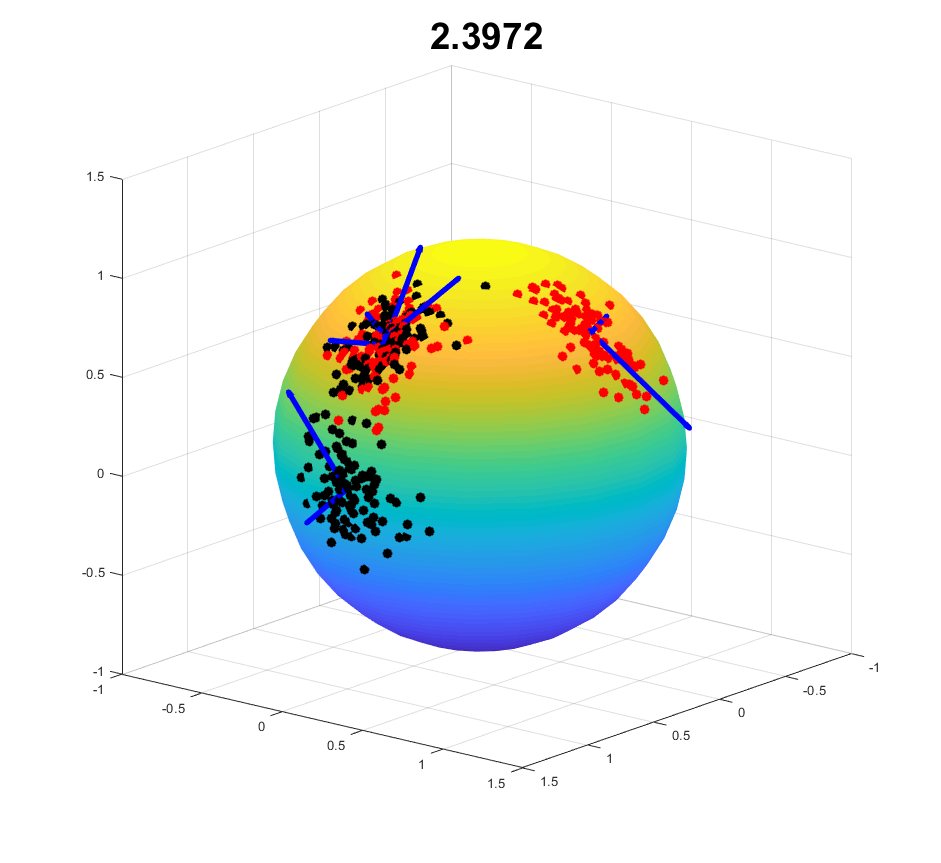
\includegraphics[width=.3\linewidth]{example6.png}
		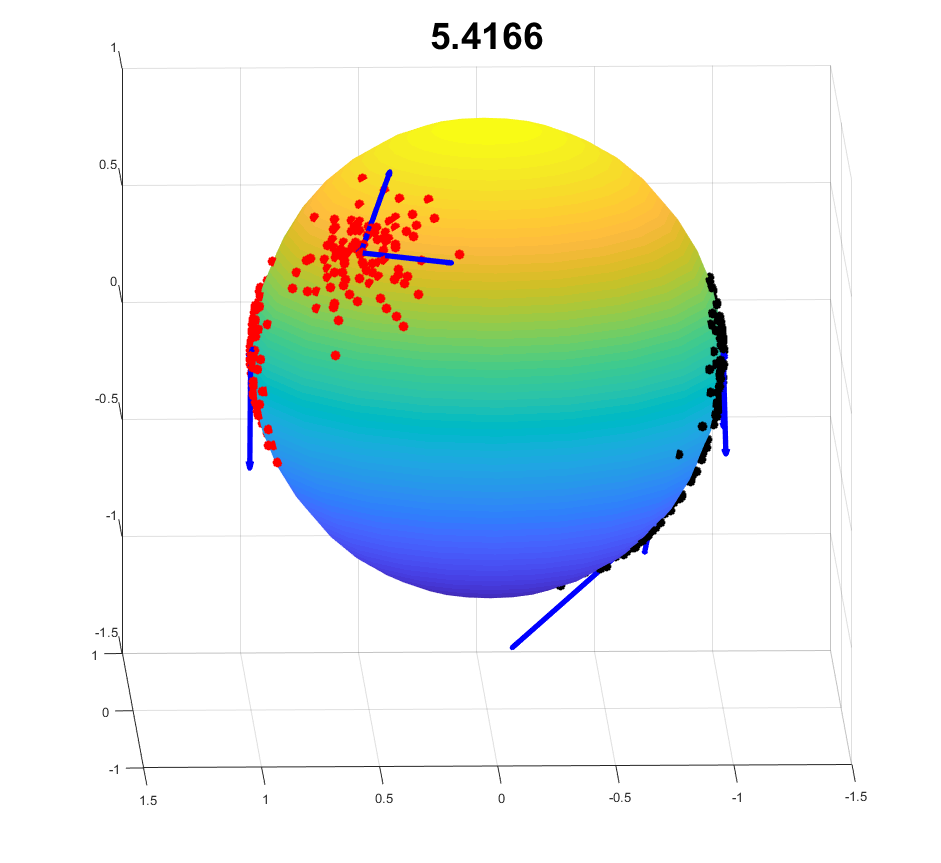
\includegraphics[width=.3\linewidth]{example8.png}
		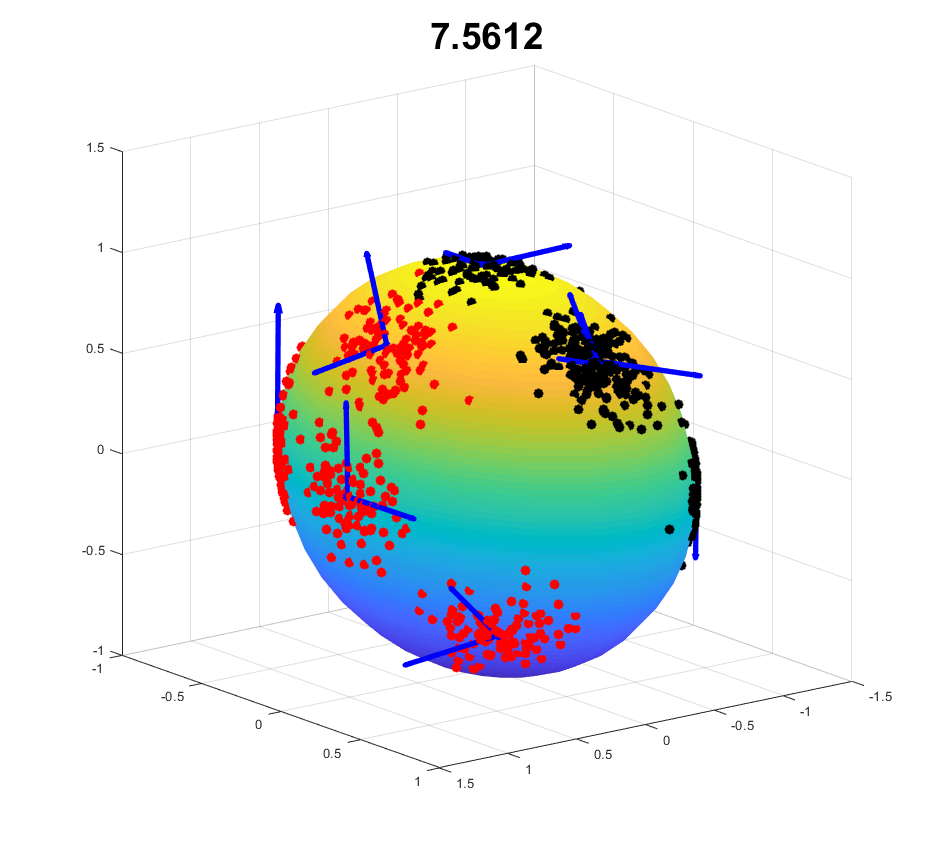
\includegraphics[width=.3\linewidth]{example10.png}
		\caption{Examples of Wrapped Gaussian Mixture Wasserstein-type distances on the sphere for simulated data}
\end{figure}

\subsection{DTMRI data}

\begin{figure}
	\begin{center}
	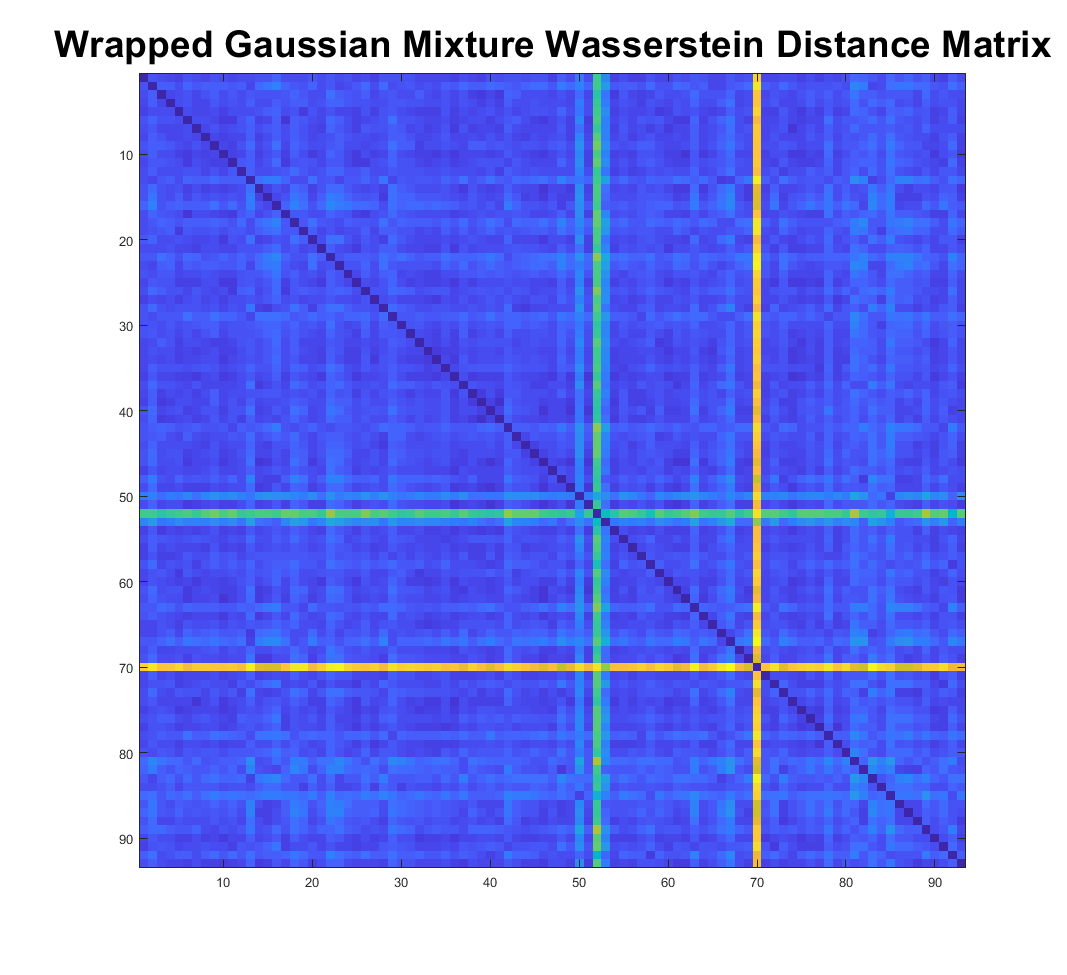
\includegraphics[width=.7\linewidth]{distance_matrix.png}
	\caption{Wrapped Gaussian Mixture Wasserstein-type Distance matrix. The first 42 columns/row correspond to non-PTSD subjects, columns/rows 43:93 correspond to PTSD subjects.  }
\end{center}
\end{figure}

One possible application of this approach is the comparison of the distributions of shapes, such as set of DTMRI fiber tracts. The data for this example consists of Fiber tractography data for the right Cingulum Parahippocampal region of 93 subjects in the Grady Trauma Project. 41 are diagnosed with PTSD, 42 are not diagnosed with PTSD. The regions are sets of fiber tracts, represented as curves in $\mathbb{R}^3$. We estimate these distributions by identifying shape modes in the shape space (using k-mode kernel mixture clustering) representing the distributions as Gaussian mixtures in the pre-shape space (which is a sphere) and then calculating the Wrapped Gaussian Mixture Wasserstein-type distance between the distributions of subjects. We then use these distances to classify subjects with respect to their PTSD status.

Specifically, let $X_i = \{ f_{ij}(t) \in L^2([0,1] \to \mathbb{R}^3), j = 1,...,M_j\}$, $i=1,...,93$ correspond to the set of fibers for subject $i$'s right Cingulum Parahippocampal region. For each $X_i$, we represent it as a wrapped Gaussian mixture $N(m_{ik}, \Sigma_{ik})$, where $m_k$ is the mode kth mode identified using the k-mode kernel mixture algorithm applied to the fibers for subject $i$, and $\Sigma_{ik}$ is the covariance of the fibers for subject $i$ assigned to cluster $k$, calculated in $T_{m_{ik}}(S^{d-1})$, the tangent space of the cluster mode in the pre-shape space. Using these as estimates for wrapped gaussian mixtures, we calculate Wasserstein-type distances using equation (\ref{eq: mixture distance}).       

The best classifier we found gets $\sim 60\%$ test set accuracy, which likely isn't significant. This could be because only a subset of mixture components is significant, causing the signal to get drowned out in the calculation of the Wasserstein distance, which takes comparisons of all mixture components down into a single number. 



\newpage

\bibliographystyle{plain}
\bibliography{refs} % Entries are in the refs.bib file

\cite{https://doi.org/10.48550/arxiv.1907.05254}
\cite{https://doi.org/10.48550/arxiv.0801.2250}
\cite{10.1307/mmj/1029003026}
\cite{COTFNT}
\cite{Ambrosio2013}
\cite{WGOT}


\end{document}

%\begin{equation}
%	W_2^2(\mu_0, \mu_1) =  \inf_{\gamma \in \gamma(\mu_0, \mu_1)} ||EX - EY|| + E||(X-EX)-(Y-EY)||  
%\end{equation}  
%
%\begin{equation}
%	= cos^{-1}(\langle m_0,m_1\rangle) + \inf_{\gamma \in \gamma(\mu_0, \mu_1)} \int_{S^{d-1} \times S^{d-1}} cos^{-1}(\langle Exp_{m_0}(R_\alpha(Exp_{m_1}^{-1}(y)), x)\rangle) \ d\gamma(x,y)
%\end{equation}
%
%\newpage

%\begin{equation}
%	= \inf_{\gamma \in \gamma(\mu_0, \mu_1)} \int_{\mathcal{X} \times \mathcal{Y}} ||x-y|| \ d\gamma(x,y) 
%\end{equation} 


%Now, since $cos^{-1}(\langle x,y \rangle) = ||Exp_{m_0}^{-1}(y) - Exp_{m_0}^{-1}(x)||$ and $R_\alpha(Exp_{m_1}^{-1}(y)) = Exp_{m_0}^{-1}(y) - Exp_{m_0}^{-1}(m_1)$, we have that
%
%\begin{equation}
%	cos^{-1}(\langle x,y \rangle) = ||R_\alpha(Exp_{m_1}^{-1}(y)) - Exp_{m_0}^{-1}(x) + Exp_{m_0}^{-1}(m_1)||
%\end{equation}
%
%Thus,
%
%\begin{equation}
%	\int_{S^{d-1} \times S^{d-1}} cos^{-1}(\langle x,y \rangle) d\gamma(x,y) = \int_{S^{d-1} \times S^{d-1}} ||R_\alpha(Exp_{m_1}^{-1}(y)) - Exp_{m_0}^{-1}(x) + Exp_{m_0}^{-1}(m_1)|| d\gamma(x,y)
%\end{equation}
%
%\begin{equation}
%	= \int_{S^{d-1} \times S^{d-1}} ||R_\alpha(Exp_{m_1}^{-1}(y)) - Exp_{m_0}^{-1}(x)\big)||  + \big\langle R_\alpha(Exp_{m_1}^{-1}(y)) - Exp_{m_0}^{-1}(x)), (Exp_{m_0}^{-1}(m_1)\big\rangle +  ||Exp_{m_0}^{-1}(m_1)|| d\gamma(x,y)
%\end{equation}
%
%\begin{multline}
%	= ||Exp_{m_0}^{-1}(m_1)||+ \int_{S^{d-1} \times S^{d-1}} ||R_\alpha(Exp_{m_1}^{-1}(y)) - Exp_{m_0}^{-1}(x)|| d\gamma(x,y) \\
%	+ \int_{S^{d-1} \times S^{d-1}} \big\langle R_\alpha(Exp_{m_1}^{-1}(y)) - Exp_{m_0}^{-1}(x)), (Exp_{m_0}^{-1}(m_1)\big\rangle d\gamma(x,y)
%\end{multline}
%
%\begin{equation}
% = cos^{-1}(\langle m_0,m_1\rangle) + \int_{S^{d-1} \times S^{d-1}} cos^{-1}(\langle Exp_{m_0}(R_\alpha(Exp_{m_1}^{-1}(y)), x)\rangle) \ d\gamma(x,y)
%\end{equation}
%
%
%
%\newpage

%
%\begin{equation}
%	= cos^{-1}(\langle m_0, m_1\rangle) + \inf_{\gamma \in \gamma(\mu_0, \mu_1)} \int_{S^{d-1} \times S^{d-1}} cos^{-1}(\big\langle x, f(y)\big \rangle) d\gamma(x,y) 
%\end{equation} 
%
%where $f(y) = Exp_{m_0} (R_\alpha( Exp_{m_1}^{-1}(y)))$, since
%
%\begin{equation}
%	R_\alpha(Exp_{m_1}^{-1}(y)) = Exp_{m_0}^{-1}(y) - Exp_{m_0}^{-1}(m_1)
%\end{equation}
%
%\begin{equation}
%	\implies ||Exp_{m_0}^{-1}(y) - Exp_{m_0}^{-1}(x) || = ||R_\alpha(Exp_{m_1}^{-1}(y)) - Exp_{m_0}^{-1}(x) + Exp_{m_0}^{-1}(m_1)||
%\end{equation}
%
%\begin{equation}
%	=  \Sigma_{i=1}^{d-1} (Exp_{m_0}^{-1}(y) - Exp_{m_0}^{-1}(x))^2 - 2(Exp_{m_0}^{-1}(y) - Exp_{m_0}^{-1}(x))(Exp_{m_0}^{-1}(m_1)) + (Exp_{m_0}^{-1}(m_1))^2 dy
%\end{equation}
%
%\begin{equation}
%	= cos^{-1}(\langle m_0,m_1\rangle) + cos^{-1}(\langle Exp_{m_0}(R_\alpha(Exp_{m_1}^{-1}(y)), Exp_{m_0}^{-1}(x))\rangle)
%\end{equation}



%Given $\mu_i = WN(m_i,\Sigma_i)$, $i = \{0,1\}$, where $m_i \in S_{d-1}$, and $\Sigma_i^{d-1 \times d-1}$, (and with densities $\rho_i$), the Wasserstein Distance between $\mu_0$ and $\mu_1$ can be calculated as;
%
%\begin{equation}\label{eq: wrapped normal wasserstein}
%	WNW_2^2(\mu_0, \mu_1) = cos^{-1}(\langle m_0, m_1 \rangle) + tr(\Sigma_0 + \Sigma_1 - 2(\Sigma_0^{\frac{1}{2}}\Sigma_1\Sigma_0^{\frac{1}{2}})^{\frac{1}{2}})
%\end{equation} 
%
%\textbf{Proof:}\\
%
%In order to prove this, we must find a continuous map $T:S^{d-1}\to S^{d-1}$ such that;
%
%1) $T$ pushes forward $\mu_0$ to $\mu_1$ ($\iff \rho_0(x) = \rho_1(Tx)|det T'|$)
%
%2) T is optimal 
%
%3) The transport cost of T is WNW\\

